\documentclass{beamer}

\usepackage[italian]{babel}
\usepackage{array}
\usepackage{hyperref}
\usepackage{graphicx}

\graphicspath{ {./images/} }

\usetheme{CambridgeUS}
\usecolortheme{orchid}
\setbeamertemplate{navigation symbols}{}

\title{Progetto di Ingegneria del software}
\author{Gruppo 13}
\institute{Universit\`a di Bologna}
\date{29 dicembre 2022}

\begin{document}

\begin{frame}
	\titlepage
\end{frame}

\begin{frame}{Indice}
	\tableofcontents
\end{frame}

\section{Il gruppo}
\begin{frame}{Il gruppo}
	\begin{itemize}
		\item Paolo Ceroni (sviluppatore front-end, UI/UX)
		\item Gabriele Crestanello (sviluppatore back-end, esperto di dominio)
		\item Mattia Girolimetto (\textbf{PO}, sviluppatore front-end \& DevOps)
		\item Federica Grisendi (sviluppatrice front-end, artista mock)
		\item Stefano Volpe (\textbf{SM}, sviluppatore-progettista back-end)
	\end{itemize}
\end{frame}

\section{Backlog di prodotto}
\begin{frame}{Backlog di prodotto (1/2)}
	\begin{table}
		\begin{tabular}{|c|c|c|c|}
			\hline
			\textbf{\#} & \textbf{Nome}             & \textbf{Punti} & \textbf{Stato} \\
			\hline
			\multicolumn{4}{|l|}{Sprint 0:``Preparazione''}                           \\
			\hline
			0           & Partita a Scrumble        & 3              & \#done         \\
			\hline
			1           & Ambiente di sviluppo CAS  & 10             & \#done         \\
			\hline
			\multicolumn{4}{|l|}{Sprint 1:``Indovina la parola (A)''}                 \\
			\hline
			2           & Configurazione tecnologie & 12             & \#done         \\
			\hline
			3           & Ambiente di test          & 16             & \#done         \\
			\hline
			4           & Classifica parole         & 15.5           & \#done         \\
			\hline
			\multicolumn{4}{|l|}{Sprint 2:``Indovina la parola (B)''}                 \\
			\hline
			5           & Parola esatta             & 39             & \#done         \\
			\hline
			6           & Analisi testuale          & 39             & \#done         \\
			\hline
		\end{tabular}
	\end{table}
\end{frame}

\begin{frame}{Backlog di prodotto (2/2)}
	\begin{table}
		\begin{tabular}{|c|c|c|c|}
			\hline
			\textbf{\#} & \textbf{Nome}           & \textbf{Punti} & \textbf{Stato}    \\
			\hline
			\multicolumn{4}{|l|}{Sprint 3:``C'\`e un tempo e un luogo per ogni cosa''} \\
			\hline
			7           & Mappa                   & 20             & \#done            \\
			\hline
			8           & Filtri temporali        & 14             & \#done            \\
			\hline
			9           & Storico partite         & 5.5            & \#done            \\
			\hline
			\multicolumn{4}{|l|}{Sprint 4:``Fantacitorio e scaTTo matto''}             \\
			\hline
			10          & Classifica politici     & 16             & \#done            \\
			\hline
			11          & Squadre Fantacitorio    & 12             & \#done            \\
			\hline
			12          & Statistiche politici    & 12             & \#done            \\
			\hline
			13          & Partite a schacchi      & 26.5           & \#done            \\
			\hline
			14          & Condivisione su Twitter & 3.5            & \#done            \\
			\hline
		\end{tabular}
	\end{table}
\end{frame}

\section{Casi d'uso}
\begin{frame}{Casi d'uso}
	\begin{figure}
		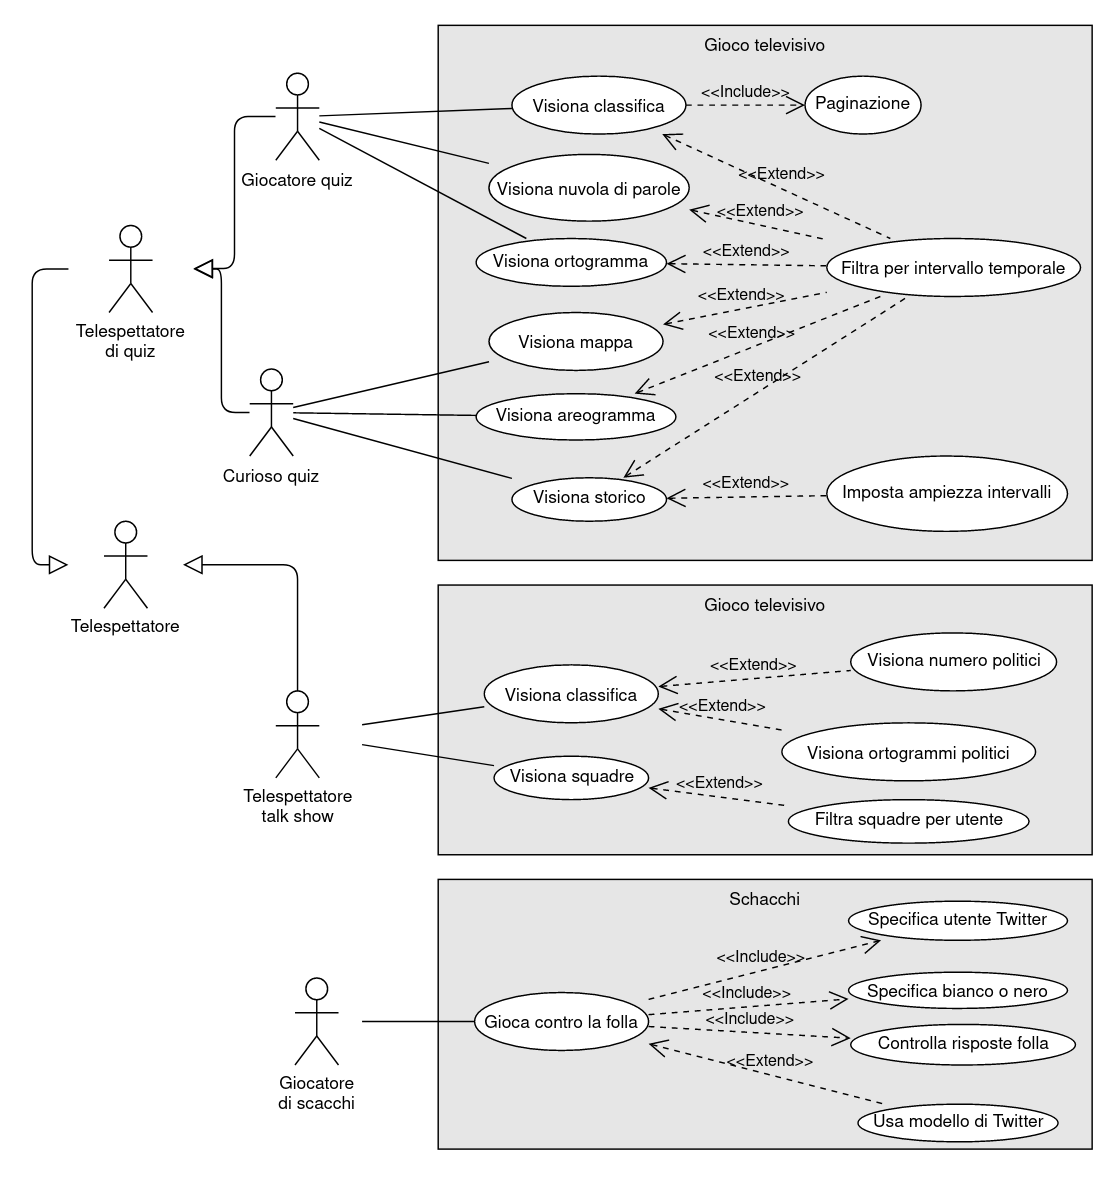
\includegraphics[width=0.5\textwidth]{use-cases}
		\caption{diagramma dei casi d'uso}
	\end{figure}
\end{frame}

\section{Diagramma dei tipi}
\begin{frame}{\texttt{model}}
	\begin{figure}
		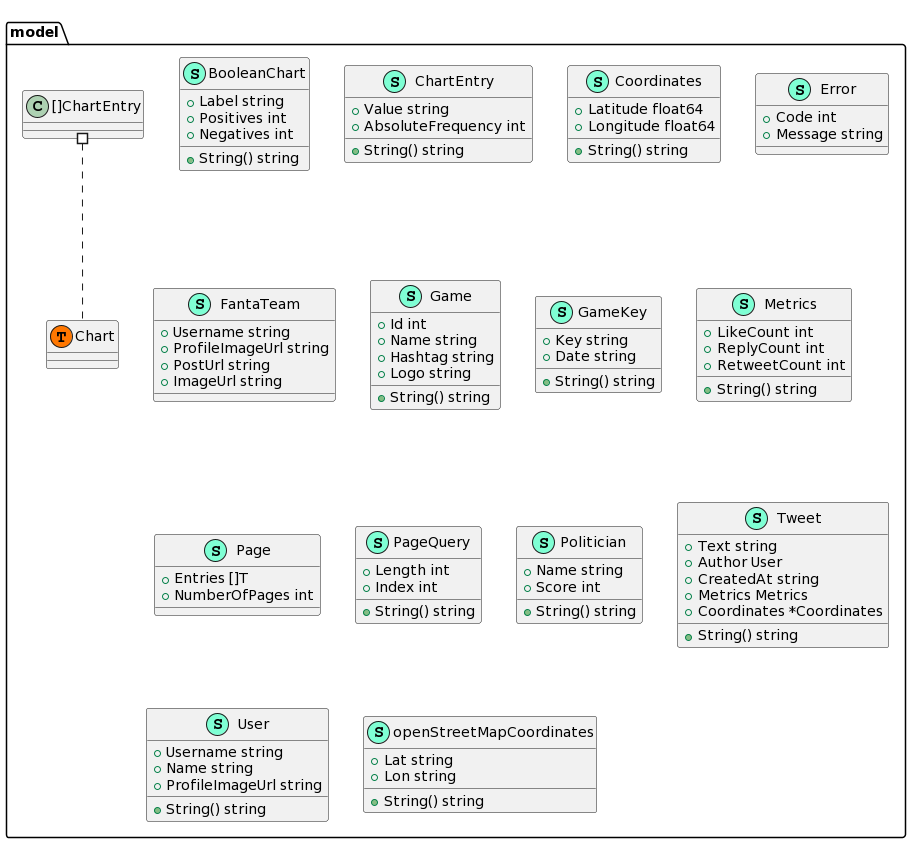
\includegraphics[width=0.6\textwidth]{backend-model}
		\caption{diagramma dei tipi di \texttt{model}}
	\end{figure}
\end{frame}

\begin{frame}{\texttt{gametracker}, \texttt{util}, \texttt{twitter},
		\texttt{fantacitorio}}
	\begin{figure}
		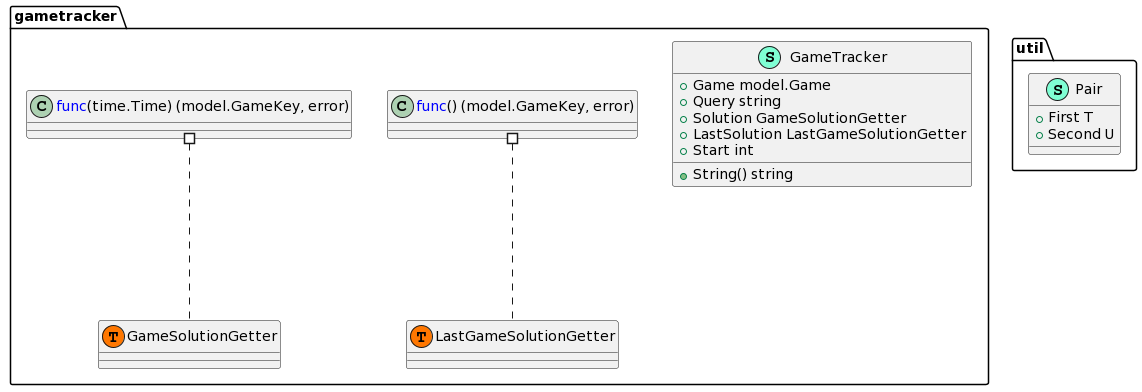
\includegraphics[width=0.6\textwidth]{backend-gametracker-util}
		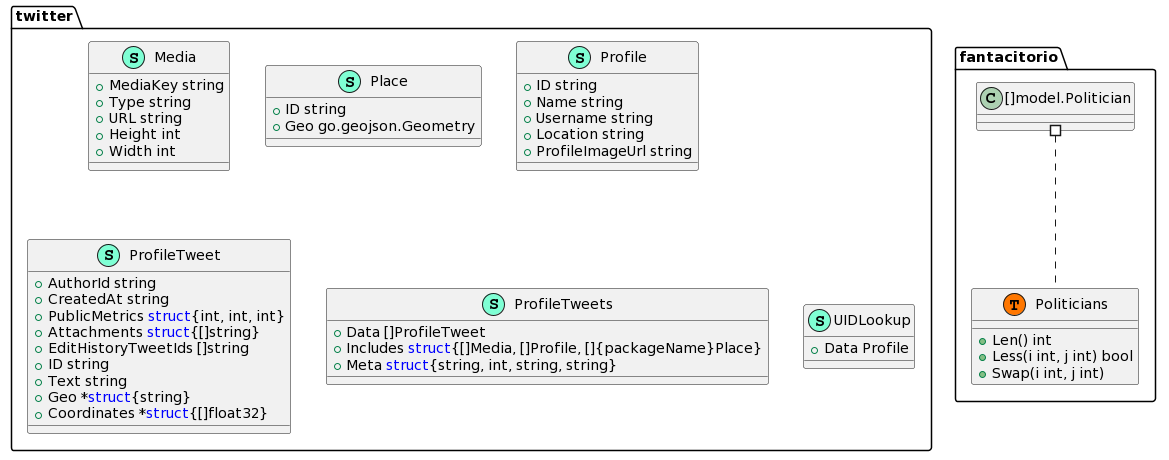
\includegraphics[width=0.6\textwidth]{backend-twitter-fantacitorio}
		\caption{diagramma dei tipi di \texttt{gametracker}, \texttt{util},
			\texttt{twitter}, \texttt{fantacitorio}}
	\end{figure}
\end{frame}

\section{Qualit\`a del codice}
\begin{frame}{Backend}
	\begin{figure}
		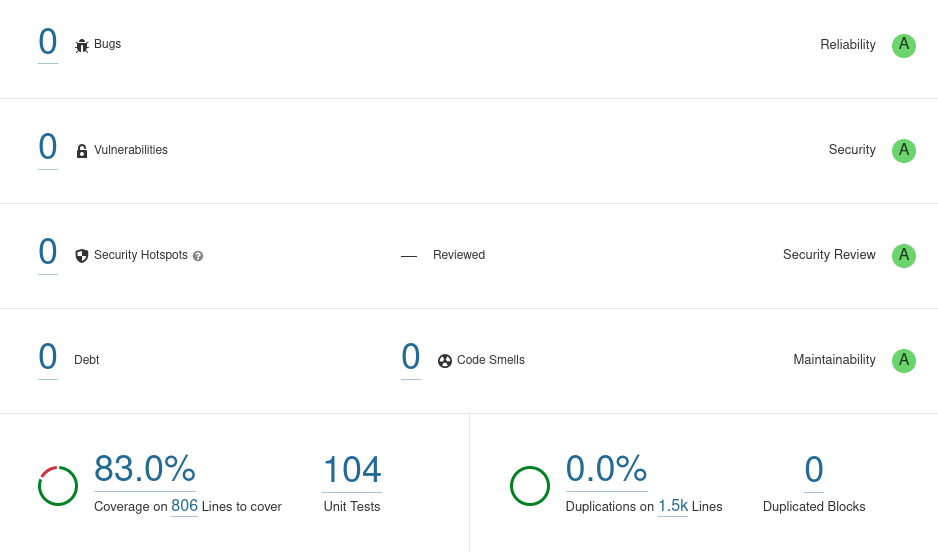
\includegraphics[width=0.8\textwidth]{quality-backend-overall}
		\caption{qualit\`a del codice backend}
	\end{figure}
\end{frame}

\begin{frame}{Frontend}
	\begin{figure}
		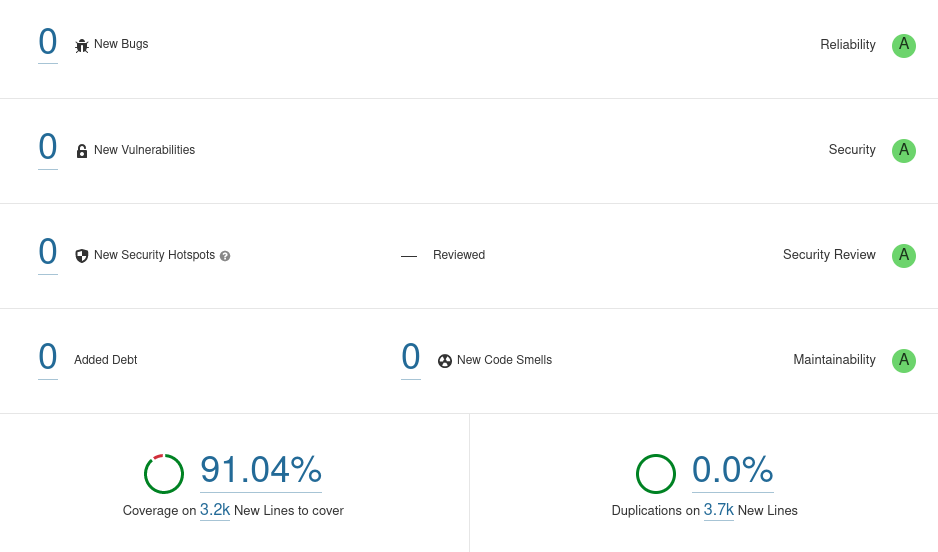
\includegraphics[width=0.8\textwidth]{quality-frontend-overall}
		\caption{qualit\`a del codice frontend}
	\end{figure}
\end{frame}

\section{Scrum}
\begin{frame}{Scrum e ludicizzazione}
	\begin{figure}
		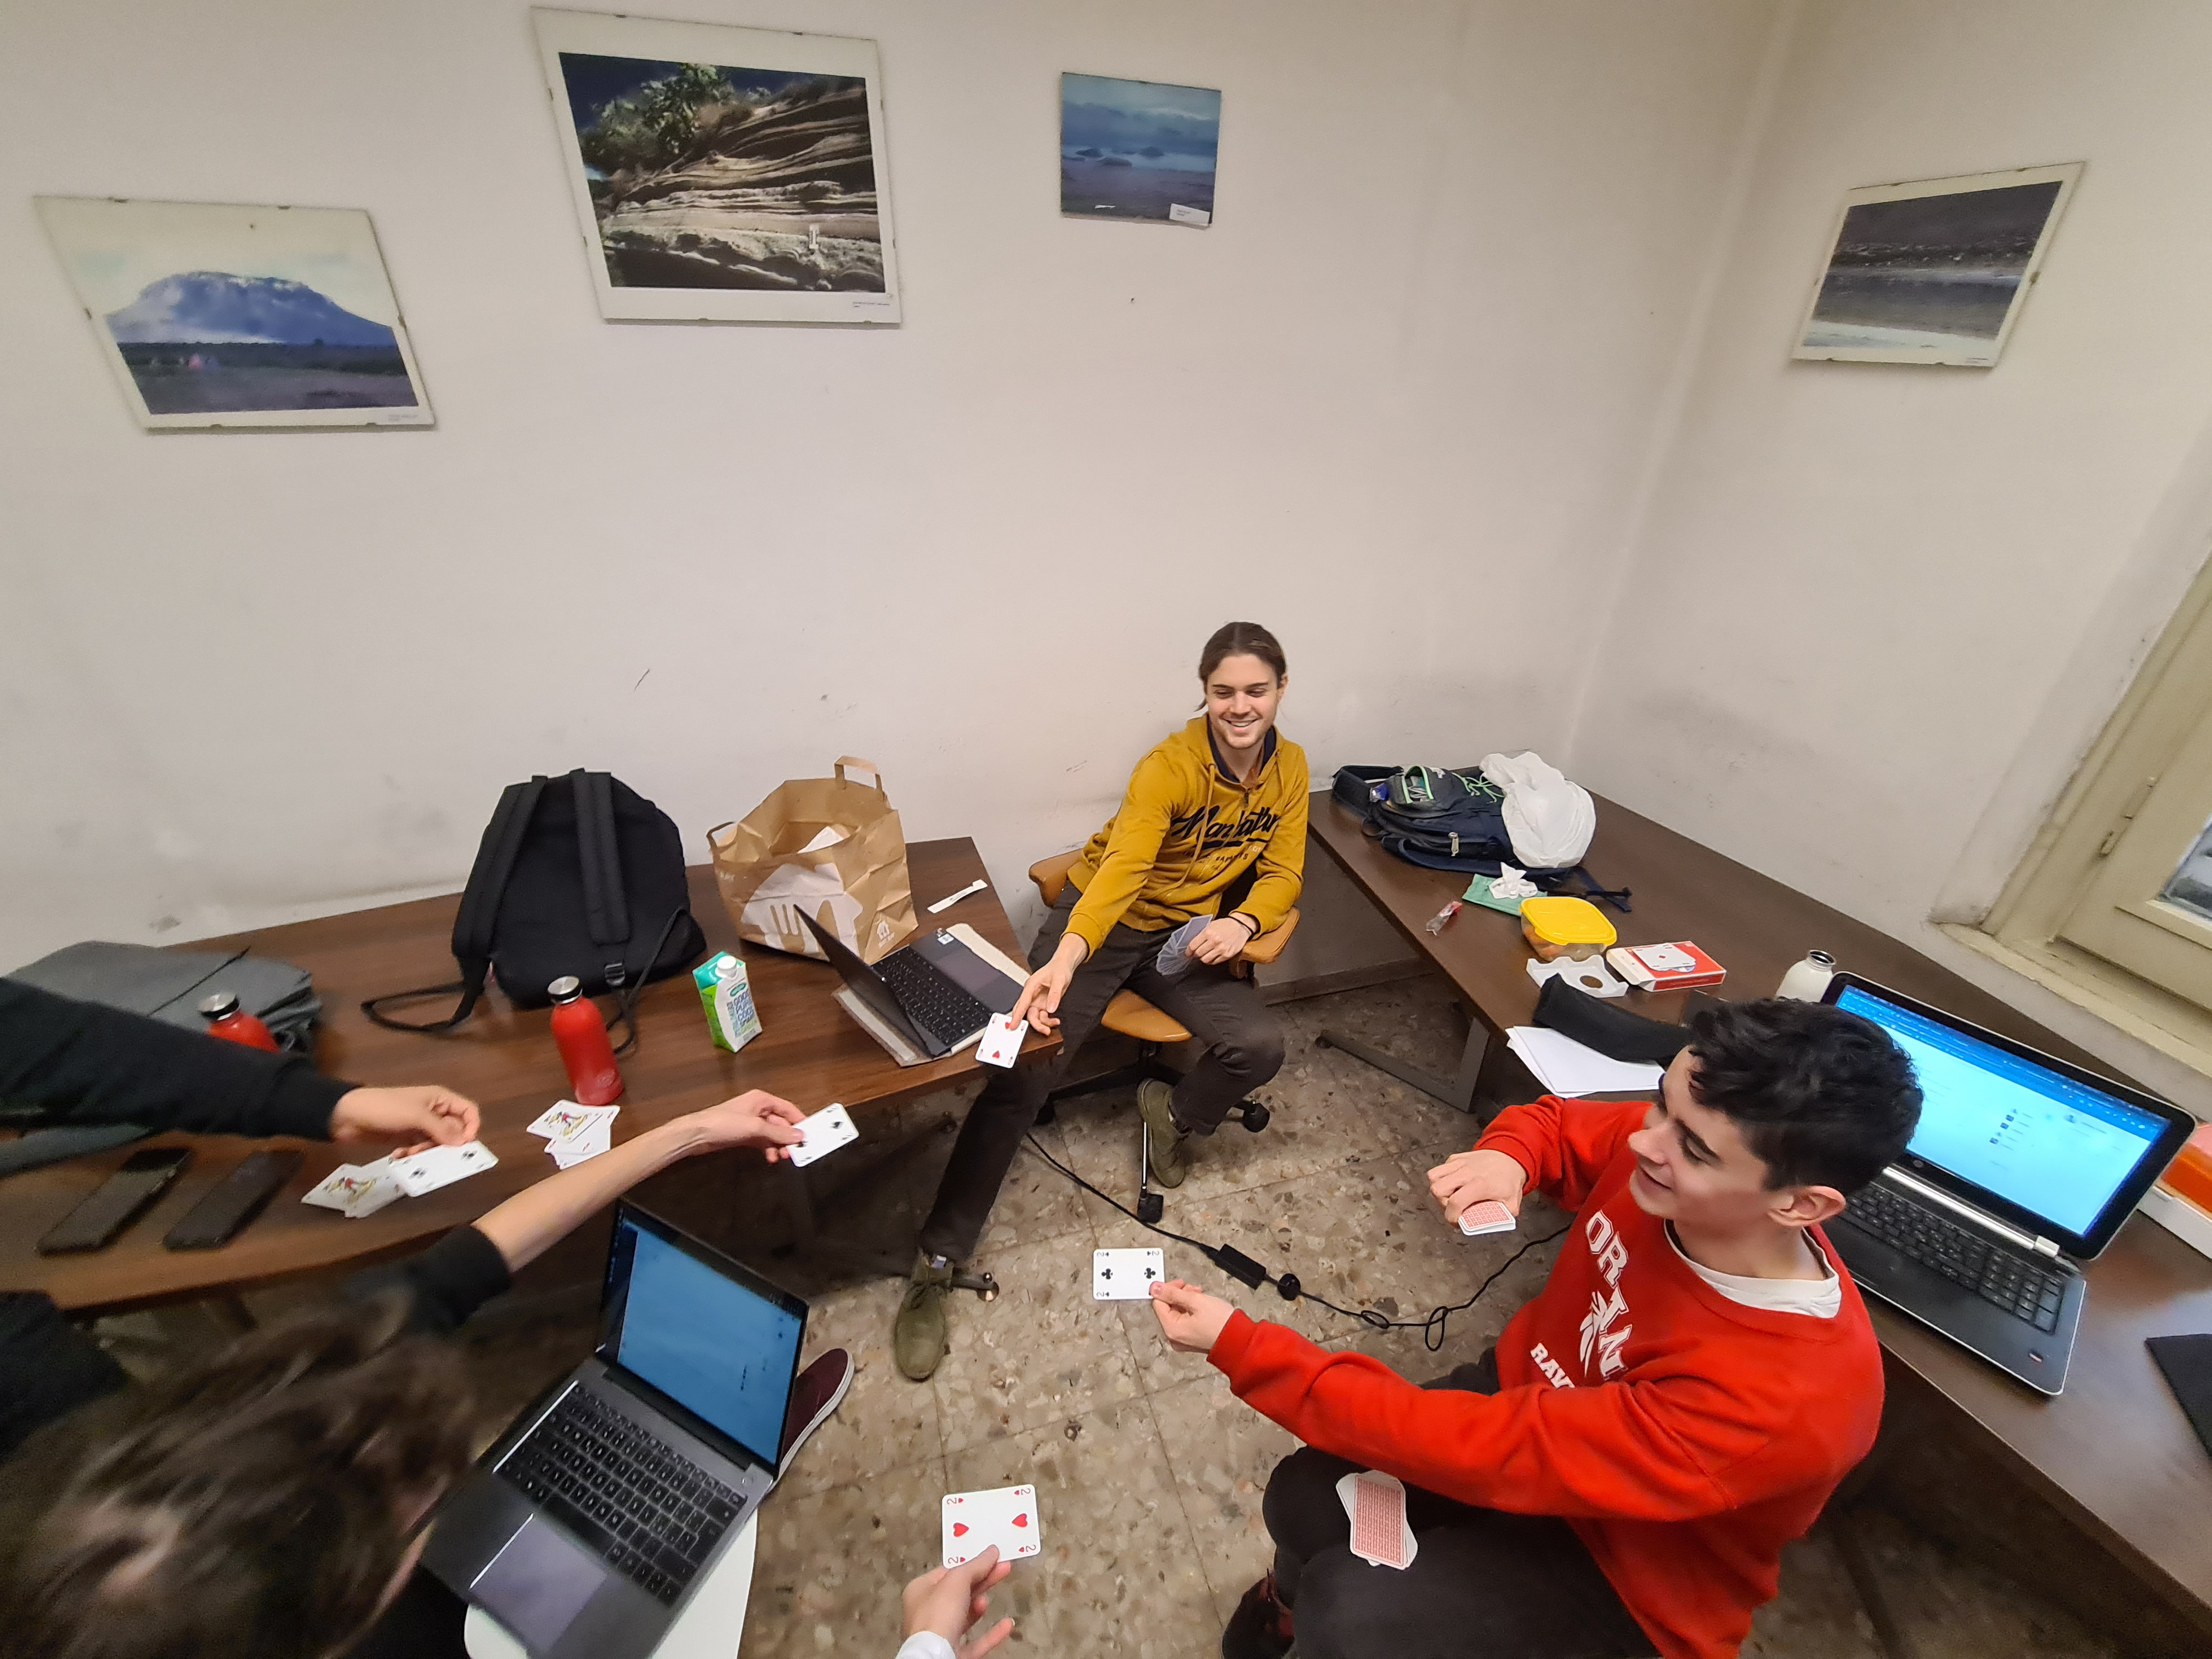
\includegraphics[width=0.35\textwidth]{planning-poker}
		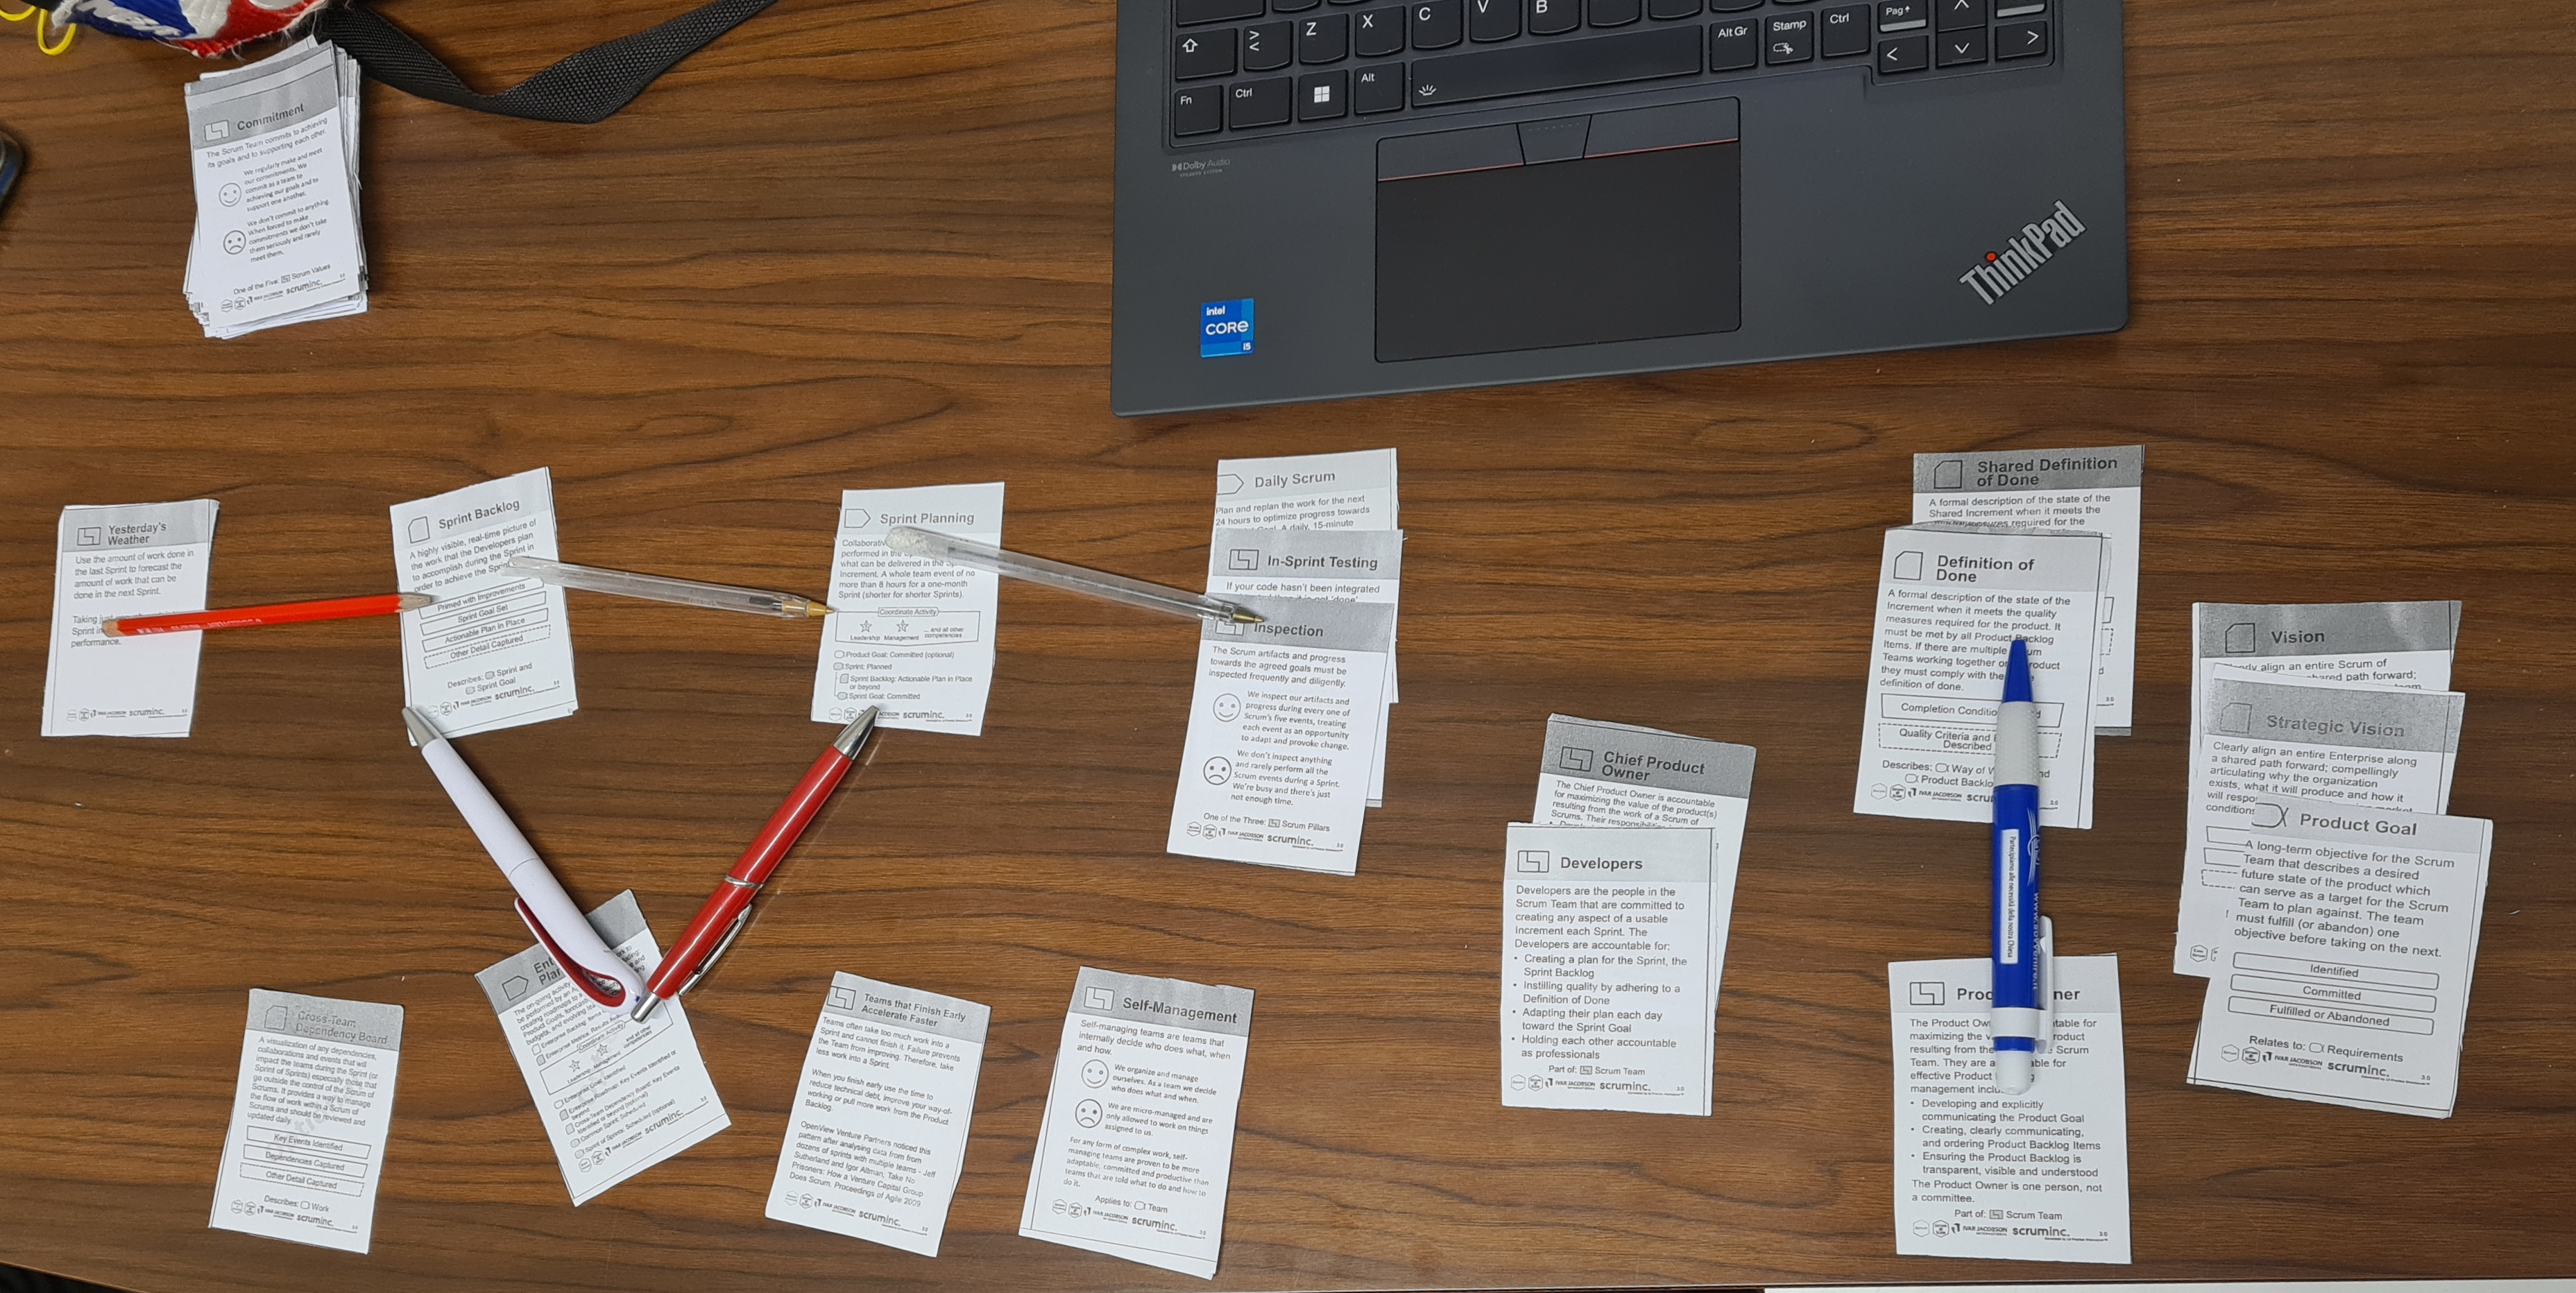
\includegraphics[width=0.45\textwidth]{essence-4-0} \\
		
\includegraphics[width=0.2\textwidth]{birdazzone-game}
		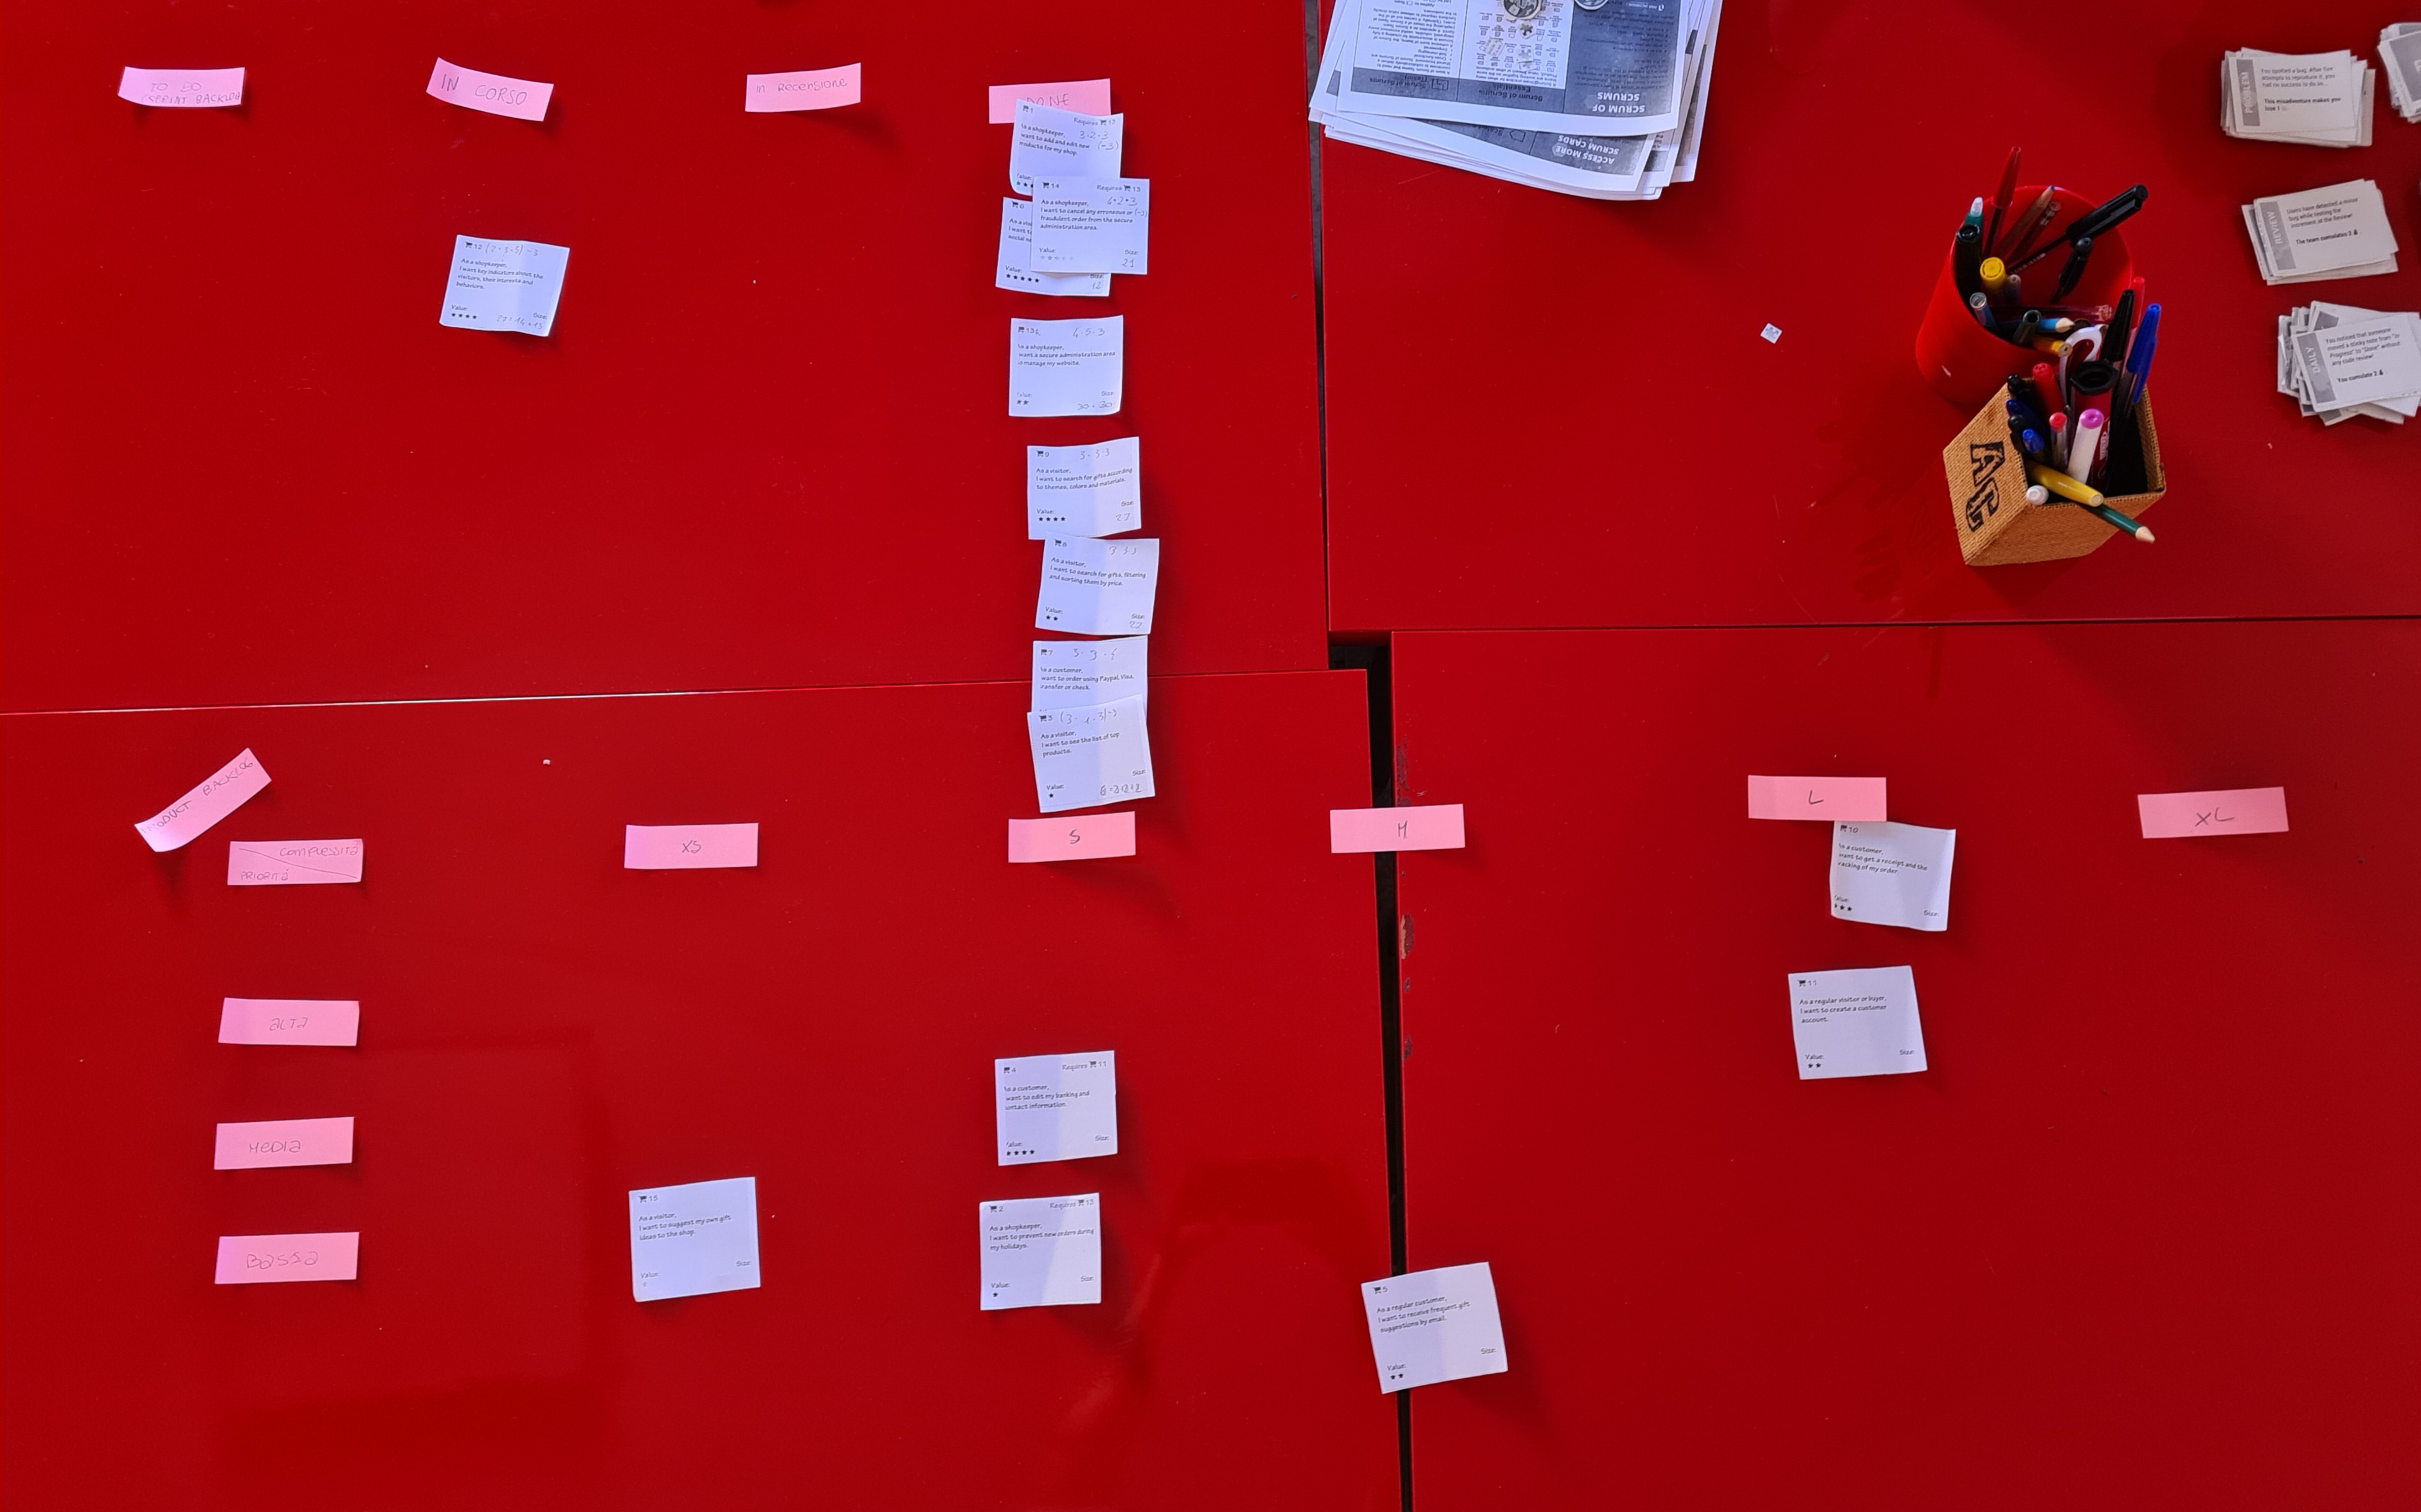
\includegraphics[width=0.35\textwidth]{scrumble}
		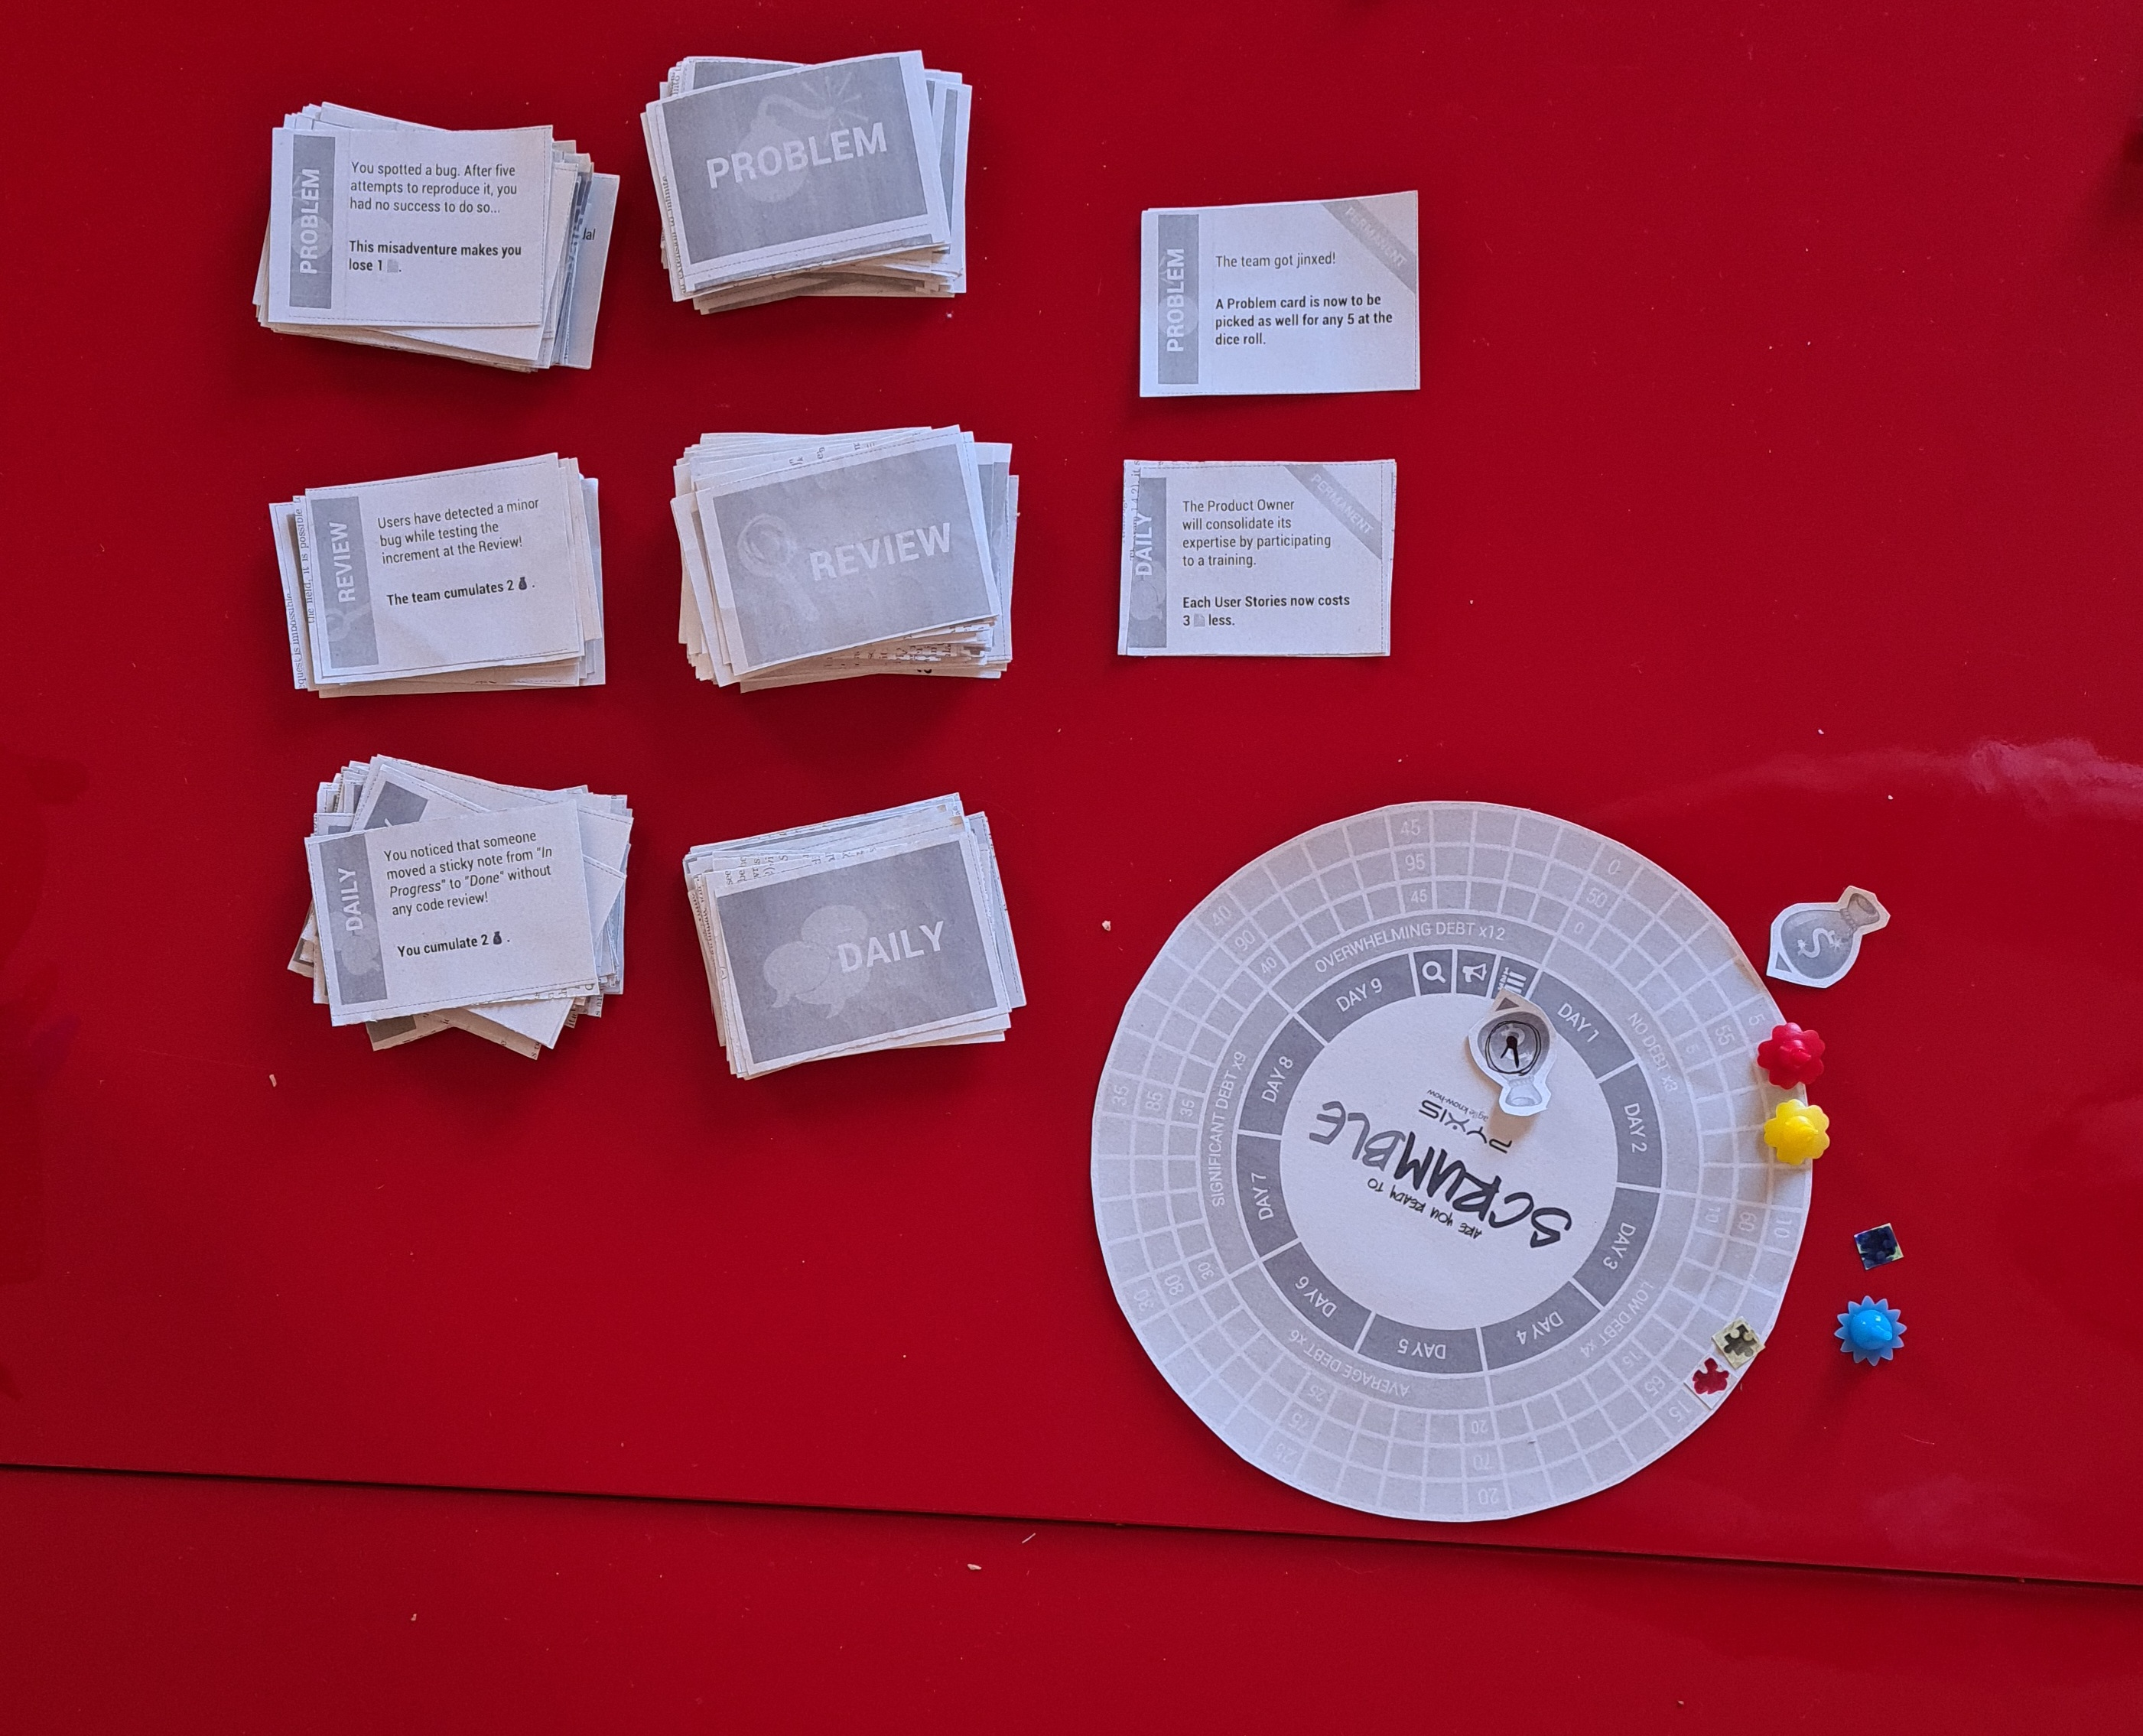
\includegraphics[width=0.25\textwidth]{scrumble-bis}
		\caption{molte delle fasi degli sprint sono state ludicizzate}
	\end{figure}
\end{frame}

\begin{frame}{Implementare la definizione di fatto}
	\begin{figure}
		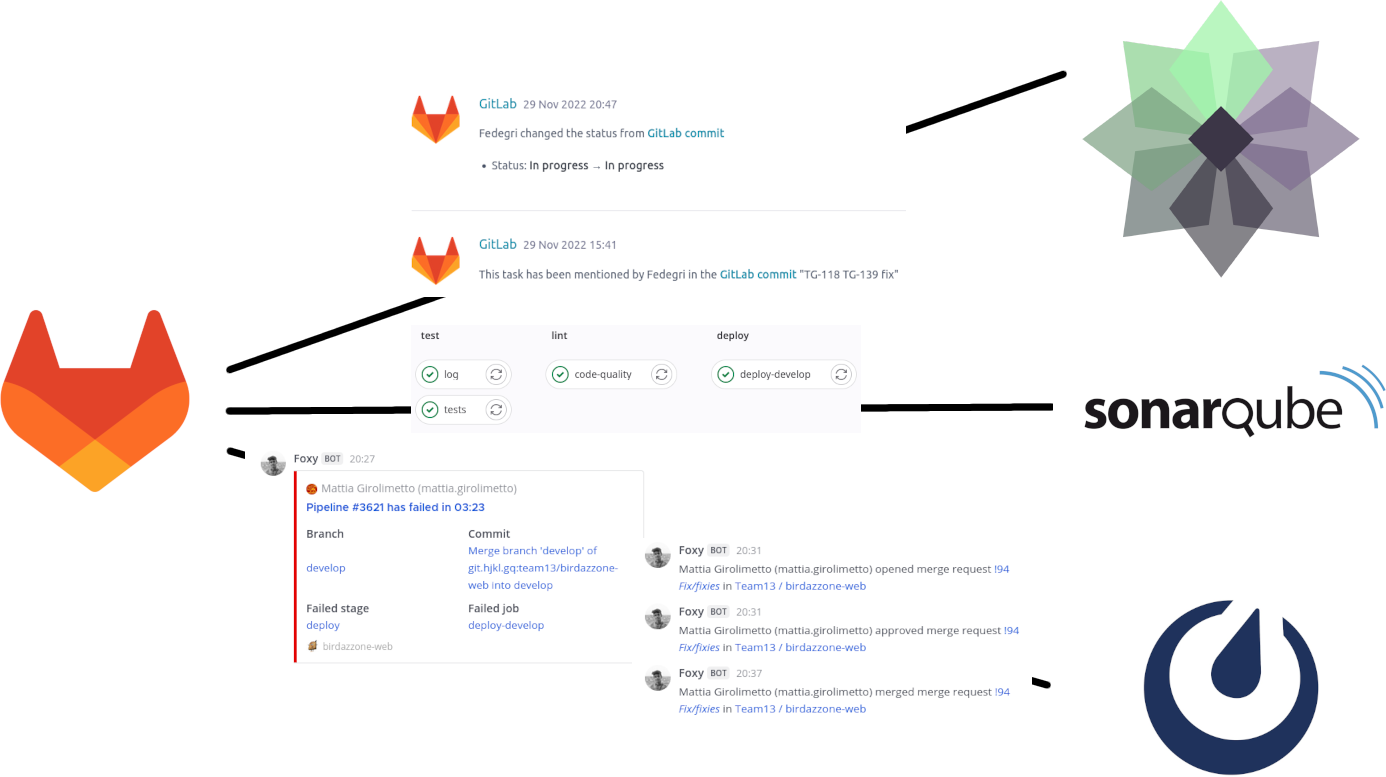
\includegraphics[width=0.8\textwidth]{integrations}
		\caption{le integrazioni automatizzate con Taiga, SonarQube e MatterMost ci
			hanno permesso di implementare controlli sulla definizione di "fatto"}
	\end{figure}
\end{frame}

\section{Retrospettiva finale}
\begin{frame}{Retrospettiva finale}
	\begin{figure}
		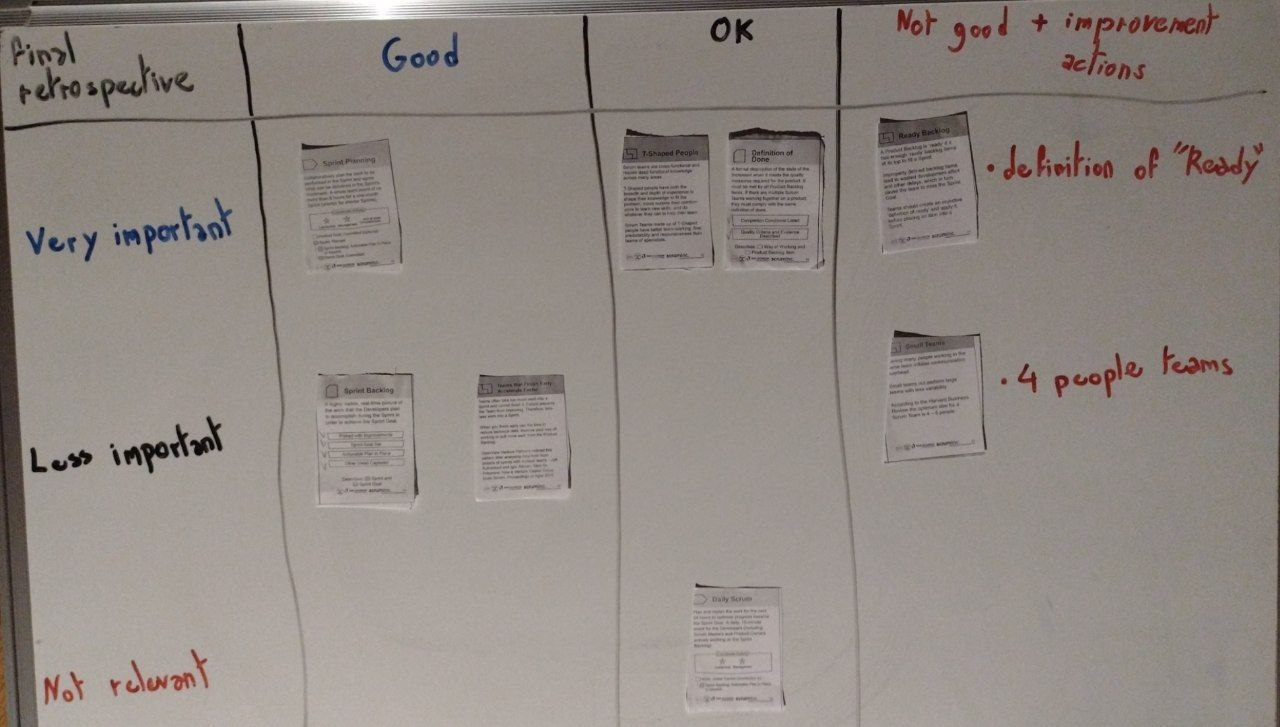
\includegraphics[width=0.9\textwidth]{essence-final}
		\caption{\emph{Patience} per la retrospettiva finale}
	\end{figure}
\end{frame}

\section{Diagramma di deployment}
\begin{frame}{Diagramma di deployment}
	\begin{figure}
		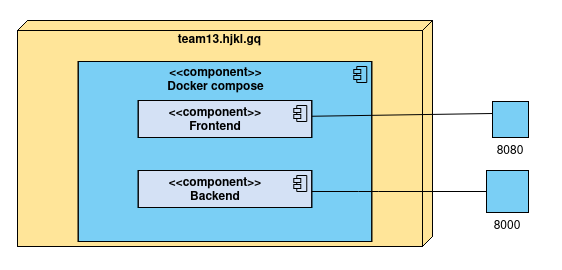
\includegraphics[width=\textwidth]{deployment}
		\caption{diagramma di deployment}
	\end{figure}
\end{frame}

\section{Demo}
\begin{frame}{Demo}
	Un'istanza privata del progetto \`e disponibile su:
	\begin{itemize}
		\item \href{http://team13.hjkl.gq:8000/swagger/index.html}{\beamerbutton{Birdazzone API}}
		\item \href{http://team13.hjkl.gq}{\beamerbutton{Birdazzone Web}}
	\end{itemize}
	Gli spazi di dipartimento non avrebbero potuto ospitarlo: offrono una gamma di
	immagini Docker troppo limitata.
\end{frame}

\end{document}
